%documentMetadata{}
\documentclass[a4paper,12pt]{article}

%\usepackage[italian]{babel}
\usepackage{pgfplots}
\usepackage{amsmath}
\usepackage{float}
\usepackage{graphicx} %for the scheme
\usepackage{array}
\usepackage[margin=1in]{geometry}
\pgfplotsset{width=10cm,compat=1.9}

\begin{document}

\parskip=10pt plus 1pt
\parindent=0pt

\begin{center}
    University of Milan

\par{\Large{Optics, Electronics, and Modern Physics Laboratory}}  

December 3, 2024 
\par


\end{center}


\par
\begin{center}
{\Large\textbf{The Michelson Interferometer}}


    
\par\noindent\rule{\textwidth}{0.4pt}

   abstract
    
    
    \par\noindent\rule{\textwidth}{0.4pt}
\end{center}



\section{Measurement of the Wavelength of Laser Light}
\subsection{Purpose and Procedure}


The objective of this experiment was to measure the wavelength of a red laser beam (\(\lambda\)) using a Michelson interferometer. The laser wavelength was determined by analyzing interference fringes produced by the recombination of two coherent light beams on a screen.  

\begin{figure}[h]
    \centering
    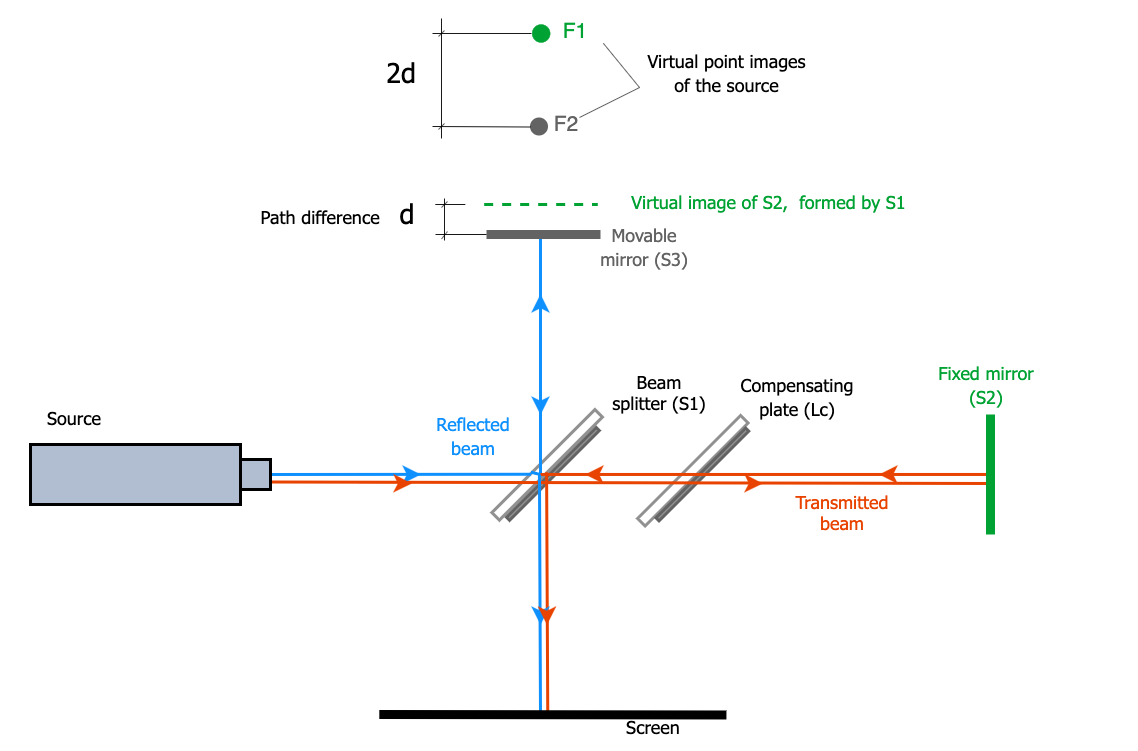
\includegraphics[width=0.9\linewidth]{The_Michelson_interferometer/finalimage1.png}
    \caption{A schematic diagram of the Michelson interferometer}
    \label{fig:michelson}
\end{figure}

The Michelson interferometer consisted of the following key components: Beam Splitter (S1) divides the incident laser beam into two orthogonal paths. Fixed Mirror (S2) reflects one of the split beams. Movable Mirror (S3) adjusted using a micrometer screw to vary the optical path difference. Compensating Plate (Lc) ensures equal optical path lengths for the two beams.  

The beam reflected by S2 traverses S1 once, while the beam reflected by S3 traverses S1 three times. The system creates two virtual coherent point sources (F1 and F2), which produce interference fringes on the screen when their light paths recombine.  

The micrometer screw controlling S3 has a sensitivity of \(2 \, \mu \text{m}\). The displacement of S3 (\(\Delta x\)) was measured as a difference between two micrometer readings, each with an uncertainty of \(2 \, \mu \text{m}\). For the wave calculation, the reflective index \(n_a\) is taken as 1, introducing a negligible error since \(n_a \approx 1.00027\). 
The wavelength was calculated using the formula:  

\[
\lambda = \frac{2 n_a\Delta x}{N} \approx \frac{2 \Delta x}{N}\,
\]  

where \(N\) is the number of fringes observed during the displacement.  

\subsection{Analysis and Error Evaluation}

The measured mirror displacements (\(\Delta x\)), fringe counts (\(N\)), and the calculated wavelengths (\(\lambda\)) are in the table below:  

\begin{table}[!htbp]
    {\par\centering
    \begin{tabular}{cccc}
        \hline
        Measure & $\Delta x \text{ (µm)}$ & $N$ & $\lambda$ \text{(nm)}\\
        \hline
        1   &   42& 130&   646.2\\
        2   &   42& 130&   646.2\\
        3   &   41& 130&   630.8\\
        4   &   40& 130&   615.4\\
        5   &   48& 130&   640.0\\
        \hline
    \end{tabular}
    \par}
    \caption{Measurement of the Wavelength of Laser Light}
\end{table}


The total uncertainty in the wavelength (\(\varepsilon_\lambda\)) arises from uncertainties in the measured displacement (\(\varepsilon_{\Delta x}\)) and the fringe count (\(\varepsilon_N\) = 1). Since \(\Delta x\) is measured as a difference of two micrometer readings, each with an uncertainty of \(2 \, \mu \text{m}\), the total uncertainty in \(\Delta x\) is:  
\[
\varepsilon_{\Delta x} = \sqrt{(2 \, \mu \text{m})^2 + (2 \, \mu \text{m})^2} = 2.83 \, \mu \text{m}
\] \[
\varepsilon_\lambda^2 = \left(\frac{\partial \lambda}{\partial \Delta x} \varepsilon_{\Delta x}\right)^2 + \left(\frac{\partial \lambda}{\partial N} \varepsilon_N\right)^2,
\] where:  \[
\frac{\partial \lambda}{\partial \Delta x} = \frac{2}{N}, \quad \frac{\partial \lambda}{\partial N} = -\frac{2 \Delta x}{N^2}.
\]

The standard deviation of the individual measurements is:  
\[
\sigma = \sqrt{\frac{\sum (\lambda_i - \bar{\lambda})^2}{n-1}} = 12.91 \, \text{nm}
\]  
The standard deviation of the mean is:  
\[
\sigma_{\text{mean}} = \frac{\sigma}{\sqrt{n}} = 5.77 \, \text{nm}
\]  


While the theoretical uncertainty is small, it only accounts for errors in \(\Delta x\) and \(N\), assuming no systematic or random errors. The standard deviation of the mean provides a more realistic estimate, capturing variability between measurements and reflecting the true precision of the experiment.  

The wavelength of the red laser was determined as:  
\[
\lambda = (636.0 \pm 5.8) \, \text{nm}
\]  

This result differs from the nominal 632.8 nm value by about 0.5\%\, indicating good agreement within 1\%\ .




\section{Measurement of the Refractive Index of Air }
\subsection{Purpose and Procedure}

This part aims to determine the refractive index of air (\(n_a\)) under laboratory conditions using a Michelson interferometer. A cylindrical air chamber of length \(D = (5.0 \pm 0.1) \, \text{cm}\) was placed in one arm of the interferometer. Initially, the chamber was evacuated (\(n_a \approx 1\)), and air was gradually reintroduced. The changes in the optical path length caused interference fringes, which were counted to calculate the refractive index.  

The refractive index was determined using the formula:  

\[
n_a = 1 + \frac{N \lambda}{2D},
\]  

where \(N\) is the number of fringes counted, \(\lambda = (635.7 \pm 5.8) \, \text{nm}\) is the laser wavelength, and \(D\) is the length of the air chamber. The uncertainties in \(n_a\) were evaluated by propagating the errors in \(N\), \(D\), and \(\lambda\).  

\subsection{Analysis and Error Evaluation}


Table 2 presents the fringe counts \((N)\), their uncertainty \((\sigma_{N})\), the calculated refractive indices \((n_a)\), and their propagated uncertainties \((\sigma_{n_a})\). Each refractive index was computed using the formula

\[
n_a = 1 + \frac{N\,\lambda}{2\,D},
\]

where \(N\), \(\lambda\), and \(D\) are measured quantities with uncertainties. The error \(\sigma_{n_a}\) for each entry was obtained via standard error propagation:

\[
(\sigma_{n_a})^2
= \left(\frac{\partial n_a}{\partial N}\right)^2 \bigl(\sigma_N\bigr)^2
+ \left(\frac{\partial n_a}{\partial \lambda}\right)^2 \bigl(\sigma_\lambda\bigr)^2
+ \left(\frac{\partial n_a}{\partial D}\right)^2 \bigl(\sigma_D\bigr)^2,
\]

with
\[
\frac{\partial n_a}{\partial N} = \frac{\lambda}{2\,D}, \quad
\frac{\partial n_a}{\partial \lambda} = \frac{N}{2\,D}, \quad
\frac{\partial n_a}{\partial D} = -\,\frac{N\,\lambda}{2\,D^2}.
\]

\begin{table}[!htbp]
    \centering
    \begin{tabular}{ccccc}
        \hline
        \text{Measure} & \({N}\) & \({\sigma_{N}}\) & \({n_a}\) & \({\sigma_{n_a}}\) \\
        \hline
        1 & 43 & 2 & 1.000273 & \(1.41\times10^{-5}\) \\
        2 & 42 & 2 & 1.000267 & \(1.40\times10^{-5}\) \\
        3 & 42 & 2 & 1.000267 & \(1.40\times10^{-5}\) \\
        4 & 41 & 2 & 1.000261 & \(1.39\times10^{-5}\) \\
        5 & 41 & 2 & 1.000261 & \(1.39\times10^{-5}\) \\
        \hline
    \end{tabular}
    \caption{Measurement of the Refractive Index of Air}
   
\end{table}

Averaging these five values gives a final refractive index:

\[
n_a = (1.000267 \pm 0.000014).
\]

The main source of error was the uncertainty in the fringe count (\(\pm 2\)). Automation of the counting process would likely improve precision. Error propagation was chosen as it properly combines the contributions from \(\sigma_{N}\), \(\sigma_\lambda\), and \(\sigma_D\), thereby accounting for both systematic and random effects.




\section{Measurement of the Coherence Length of White and Green Light}
\subsection{Purpose and Procedure}

The objective of this part was to measure the coherence length (\(L_c\)) of white and green light using a Michelson interferometer. The light sources emit wave packets with finite lengths, resulting in a measurable range of fringe visibility. After initially aligning the interferometer with a laser at zero optical path difference, the laser was replaced by the white or green light source. The movable mirror (S3) was then adjusted slowly and the difference between two recorded positions (\(x_0\) and \(x\)) was noted. Due to a mechanical lever ratio, the actual mirror displacement is one-fifth of \(|x_0 - x|\). Thus, the range (\(\Delta x\)) over which the fringes remained visible corresponds to \(|x_0 - x|/5\), and this effective displacement is the coherence length of the respective light source:

\[
L_c = \Delta x.
\]

The procedure was repeated for both white and green light.

\subsection{Analysis and Error Evaluation}

The measured values of \(x_0\), \(x\), and \(\Delta x\) for the coherence length of white and green light are in the tables below:  

\begin{table}[!htbp]
    {\par\centering
    \begin{tabular}{cccc}
        \hline
        Measure & $ x_0 \text{ (µm)}$ & $x \text{ (µm)}$ & $\Delta x$ \text{(µm)}\\
        \hline
        1   &   8690& 8750&   12\\
        2   &   8680& 8750&   14\\
        3   &   8770& 8670&   20\\
        4   &   8680& 8750&   14\\
        5   &   8690& 8730&   8\\
        6   &   8680& 8740&   12\\
        \hline
    \end{tabular}
    \par}
    \caption{Measurement of the Coherence Length of White Light }
\end{table}

\begin{table}[!htbp]
    {\par\centering
    \begin{tabular}{cccc}
        \hline
        Measure & $ x_0 \text{ (µm)}$ & $x \text{ (µm)}$ & $\Delta x$ \text{(µm)}\\
        \hline
        1   &   8650& 8790&   28\\
        2   &   8640& 8780&   28\\
        3   &   8650& 8780&   26\\
        4   &   8780& 8650&   26\\
        \hline
    \end{tabular}
    \par}
    \caption{Measurement of the Coherence Length of Green Light }
\end{table}

The mean coherence length for white light and the standard deviation of the mean:
\[
L_c,w = (13.33 \pm 1.83) \, \mu \text{m}
\]  
The mean coherence length for green light and the standard deviation of the mean:
\[
L_c,g = (27.00 \pm 0.71) \, \mu \text{m}
\]  

The main difficulty encountered was the precise determination of the point at which fringes disappear. This led to some variability in the measurements.


\section{Measurement of the Separation of Sodium Doublet Lines}
\subsection{Purpose and Procedure}
 

The final part of the experiment involves replacing the light source with a sodium lamp. The purpose of this experiment was to measure the separation between the two sodium D-lines, which are closely spaced at approximately 6 Å (\(\lambda_1 = 5890 \, \text{Å}\) and \(\lambda_2 = 5896 \, \text{Å}\)). The sodium light source was introduced into the Michelson interferometer, and the interference fringes produced by the two closely spaced wavelengths were analyzed.

A diaphragm and converging lens were placed between the sodium lamp and the beam splitter to filter and focus the light. This setup helped create a sharp interference pattern on the screen. The movable mirror (S3) was adjusted to measure the displacement (\(\Delta x\)) corresponding to one modulation cycle. This displacement was used to calculate the separation of the sodium doublet lines using the formula:

\[
\Delta \lambda = \frac{m \lambda^2}{2 \Delta x}
\]

Where:
 \(\lambda = 5893 \, \text{Å}\) is the average wavelength of the sodium D-lines,
 \(m\) is the number of sharp interference pattern transitions observed (for this experiment, \(m = 5\)),
 \(\Delta x\) is the displacement measured during the experiment.
\subsection{Analysis and Error Evaluation}

The measured values of \(x_0\), \(x\), and \(\Delta x\) for the separation of the sodium D-lines: 

\begin{table}[!htbp]
    {\par\centering
    \begin{tabular}{cccc}
        \hline
        Measure & $ x_0 \text{ (µm)}$ & $x \text{ (µm)}$ & $\Delta x$ \text{(mm)}\\
        \hline
        1   &   8060& 3790&   0.85 \\
        2   &   6600& 13650&  1.41 \\
        3   &   2300& 10700&  1.68 \\
        4   &   5180& 12110&  1.39 \\
        5   &   6620& 13610&  1.40 \\
        6   &   8090& 15070&  1.40 \\
        \hline
    \end{tabular}
    \par}
    \caption{Measurement of the Separation of Sodium Doublet Lines }
\end{table}

From these measurements, the average mirror displacement is
\[
\overline{\Delta x} = (1.355 \pm 0.111)\,\text{mm}
\]

In formula for \(\Delta \lambda\), \noindent
$m$ is an integer count of modulation cycles (assumed exact), and 
$\lambda$ is taken from the literature with negligible uncertainty relative to that of $\Delta x$. Therefore, the main source of uncertainty in 
$\Delta \lambda$ comes from $\Delta x$.

\medskip

To propagate the uncertainty, we note that

\[
\varepsilon_{\Delta \lambda}^2 = \left(\frac{\partial \Delta \lambda}{\partial \Delta x}\varepsilon_{\Delta x}\right)^2
\], leading to
\[
\varepsilon_{\Delta \lambda} = \left|-\frac{m \lambda^2}{2 \Delta x^2}\right|\varepsilon_{\Delta x} = \frac{m \lambda^2}{2 \Delta x}\frac{\varepsilon_{\Delta x}}{\Delta x}=\Delta \lambda \frac{\varepsilon_{\Delta x}}{\Delta x}
\]
%It is often convenient to express the relative uncertainties. Since \(\Delta \lambda \propto \frac{1}{\Delta x}\):

%\[
%\frac{\varepsilon_{\Delta \lambda}}{\Delta \lambda} = \frac{\varepsilon_{\Delta x}}{\Delta x}.
%\]

%This shows the relative uncertainty in \(\Delta \lambda\) is the same as that in \(\Delta x\).

%Assume the measured mean displacement is \(\bar{\Delta x} = (1.43 \pm 0.07)\,\text{mm}\). The relative uncertainty in \(\Delta x\) is \(\varepsilon_{\Delta x}/\Delta x = 0.07/1.43 \approx 0.049 \) (approximately 4.9%).

%From the measured data, substituting \(\bar{\Delta x} = 1.43\,\text{mm}\), \(\lambda = 5893\,\text{Å}\), and \(m = 5\):

%\[
%\Delta \lambda = \frac{5 \times (5893\,\text{Å})^2}{2 \times 1.43\,\text{mm}}.
%\]

%Evaluating the numerator and keeping consistent units, yields approximately

Since \(\Delta \lambda = 6.41\, \text{Å}\) and \(\varepsilon_{\Delta x}/\Delta x = 0.082\), the absolute uncertainty is

\[
\varepsilon_{\Delta \lambda} =  6.41\,\text{Å} \times 0.082 \approx 0.53\,\text{Å}
\]

The final result for separation of the sodium D-lines is

\[
\Delta \lambda = (6.41 \pm 0.53)\,\text{Å}
\]

This result is in good agreement with the known separation of about 6 Å between the sodium D-lines. The dominant uncertainty arises from the measurement of \(\Delta x\). By using standard error propagation, the final uncertainty in \(\Delta \lambda\) is realistically estimated.






\section{Conclusion}
 
The laser wavelength, the refractive index of air, the coherence lengths of white and green light, and the separation of the sodium D-lines are in good agreement with known or expected values. The use of appropriate error analysis methods, combining statistical treatment of repeated measurements with proper error propagation for derived quantities, ensured realistic uncertainty estimates. 
Difficulties primarily arose in accurate fringe counting, especially when large numbers of fringes were involved or when aligning the interferometer to achieve stable interference patterns. The micrometer screw exhibited slight play, though consistently turning it in the same direction mitigated this issue. Despite these challenges, the experimental methods proved robust, and the selected error estimation approaches — statistical for multiple measurements and partial-derivative propagation for single-step calculations accounted for both random and systematic uncertainties.


\end{document}
